\section{Analysis}
\subsection{Functional Requirements and Use Cases}
\subsubsection{Use Cases List}
\begin{itemize}
	\item An \textit{unregistered user} can
	\begin{itemize}
		\item Register
	\end{itemize}
	\item A \textit{registered user} can
	\begin{itemize}
		\item Login
		\item Consult \textit{Pokèdex}
		\begin{itemize}
			\item Search by \textit{Name}
			\item Search by \textit{Type(s)}
			\item Search by \textit{Pokédex ID}
			\item Search by \textit{Catch Rate}
			\item Search by \textbf{Pokemon} characteristics like \textit{Height} or \textit{Weight}
		\end{itemize}
		\item Consult \textit{Ranking}:
		\begin{itemize}
			\item Most popular \textbf{Pokèmon} among all \textbf{Users}
			\item Most popular \textbf{Pokèmon} in each \textit{Country}
			\item Best World \textbf{Teams}
			\item Best Teams among Friends
			\item Best Teams by \textit{Country}
		\end{itemize}
		\item Find \textbf{Users}:
		\begin{itemize}
			\item See recommended \textbf{Users} based on common friends
			\item See recommended \textbf{Users} based on common Pokémon interests
			\item Find \textbf{Users} by \textit{username}
			\item Follow/Unfollow them
		\end{itemize}
		\item Interact with \textbf{Pokèmon} network:
		\begin{itemize}
			\item Insert/Remove a \textbf{Pokémon} in his/her own favourite Pokémon list
			\item Create a \textbf{Post} on a \textbf{Pokémon} to share opinions
			\item Add answers to \textbf{Posts}
			%\item Follow/Unfollow them
			\item The post owner can also remove the \textbf{Post} at his/her will
		\end{itemize}
		\item \textbf{Team} handling:
		\begin{itemize}
			\item Remove \textbf{Pokemon} from the \textbf{Team}
			\item View \textbf{Team}
			\item Change name of the \textbf{Team}	
			\item Save modified \textbf{Team}
			\item View the value of the \textbf{Team}
		\end{itemize}
		\item Catching:
		\begin{itemize}
			\item Browse a \textbf{Pokémon} you want to catch searching it by \textit{name} 
			\item Select a \textbf{Pokémon} you want to catch from the list of favourites
			\item Try to catch a \textbf{Pokemon} to add to your \textbf{Team}
		\end{itemize}
		\item \textit{Settings}:
		\begin{itemize}
			\item Change \textit{Email}
			\item Change \textit{Password}
			\item Change \textit{Country}
		\end{itemize}
		\item Logout:
		\begin{itemize}
			\item Exit from the account
			\item Return to the sign in window
		\end{itemize}
		\item At each time can:
		\begin{itemize}
			\item See her/his \textit{username}
			\item See the remaining \textit{daily Pokèballs}
			\item Mute/Unmute Music
		\end{itemize}
		\item At each time a \textit{pokèmon name} is visible:
		\begin{itemize}
			\item By clicking on a \textit{Pokémon name}, visualize all the information about it
		\end{itemize}
		\item At each time a \textit{username} is visible
		\begin{itemize}
			\item By clicking in a \textbf{User}’s \textit{username}, visualize all the information about his/her \textbf{Team}
		\end{itemize}
	\end{itemize}
	\item An \textit{admin} can
	\begin{itemize}
		\item Sign In
		\item Add \textbf{Pokèmon} to the \textit{Pokédex}
		\item Remove \textbf{Pokèmon} from \textit{Pokédex}
		\item See the number of registered \textbf{Users} in time
		\item See the numbers of login per day
		\item See the numbers of login per day in every \textit{Country}
		\item Remove a \textbf{User} from the system
		\item Remove \textbf{Posts/Answers} from the system
		\item Consult \textit{Rankings}
		\item Logout
\end{itemize}
	\item The \textit{system} should
	\begin{itemize}
		\item Daily update Pokeball number of each \textbf{User}
		\item Periodically update \textbf{Pokèmon} \textit{catch rates} based on the number of users that own that \textbf{Pokèmon}
		\item Update \textbf{Team} points if the \textbf{User} has six \textbf{Pokémons} of different \textit{types}
		\item Periodically compute usage statistics to be consulted by the administrators
	\end{itemize}
\end{itemize}

\subsubsection{UML Use Cases Diagram}
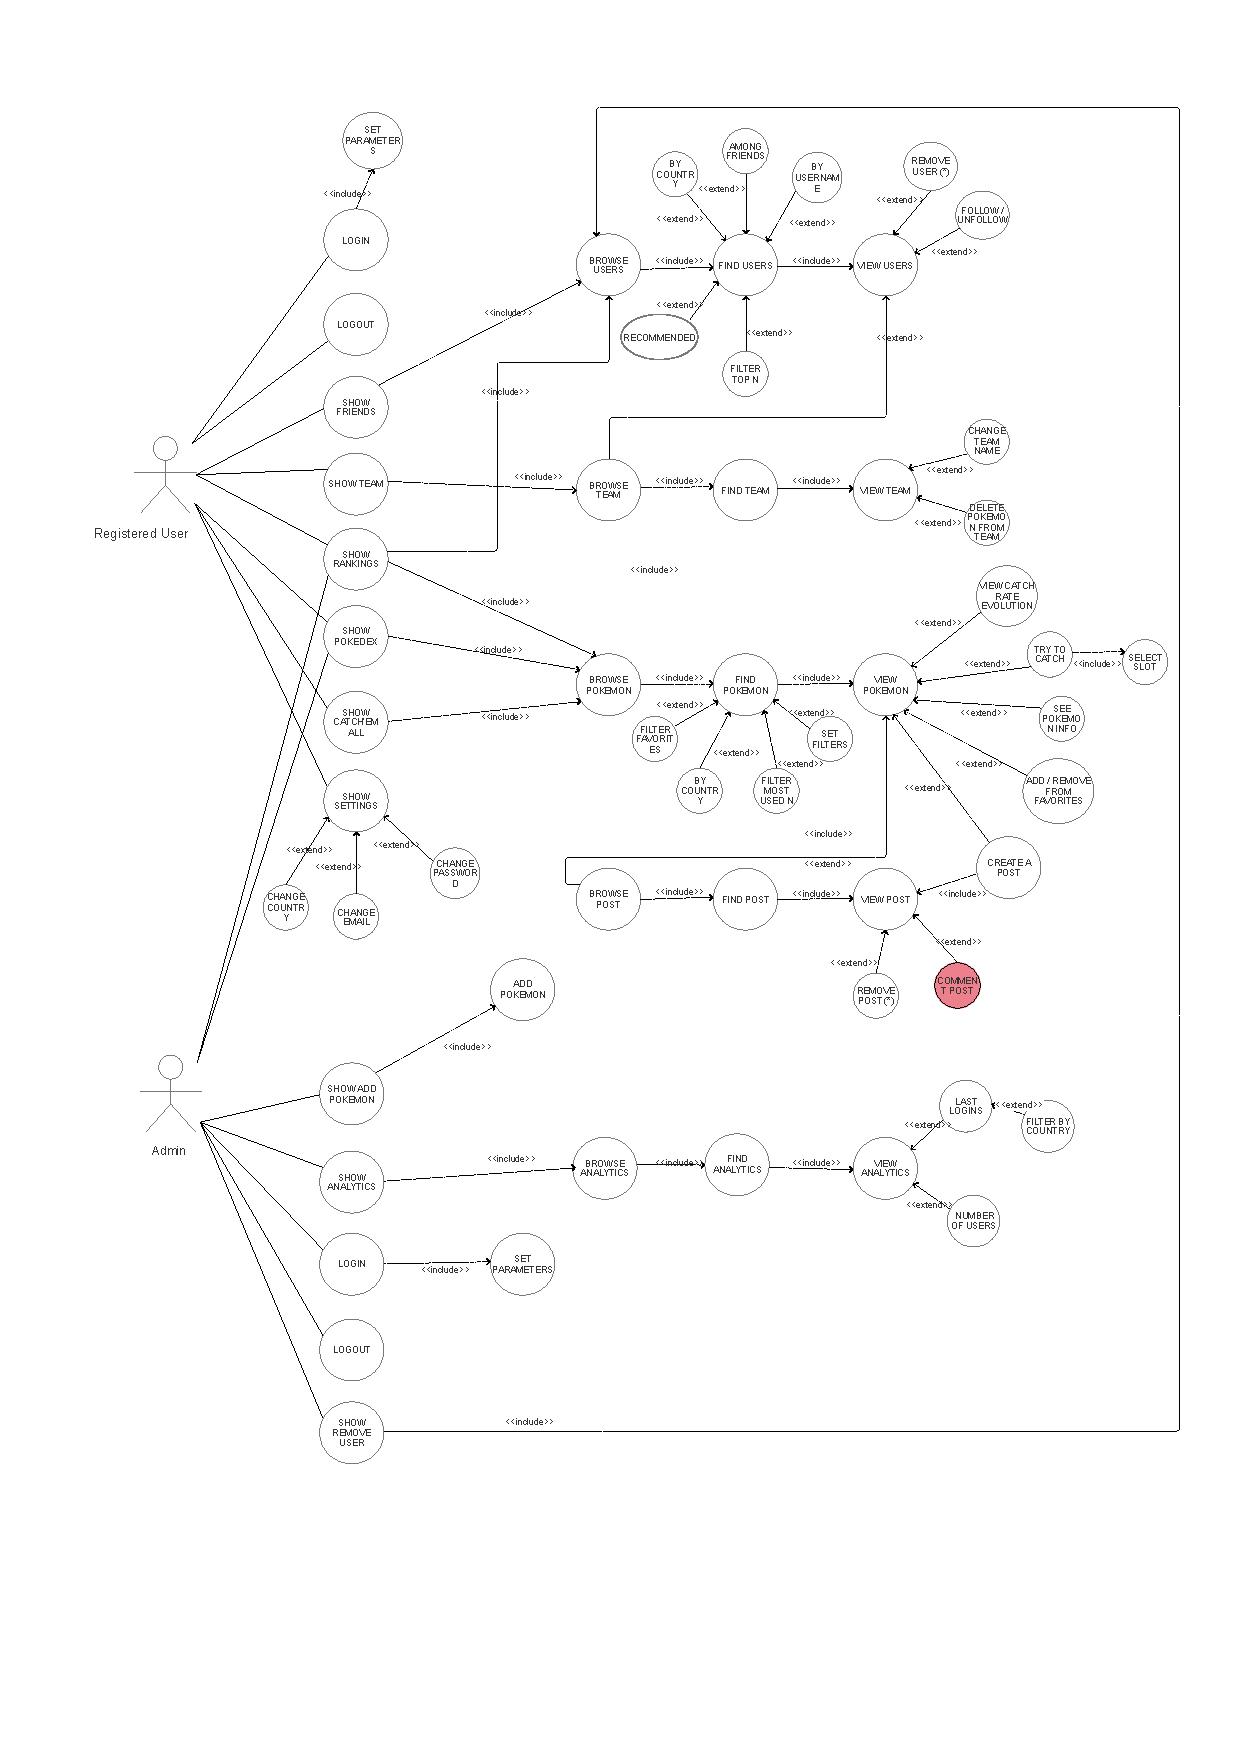
\includepdf{img/uml_use_case_1.pdf}
\begin{figure}[H]
	\caption{Use Case Diagram 1\\ (*) only for the User who created the Post and Admins, in red Browse-find-view comments had not been reported )}

\begin{figure}[H]
	\centering
	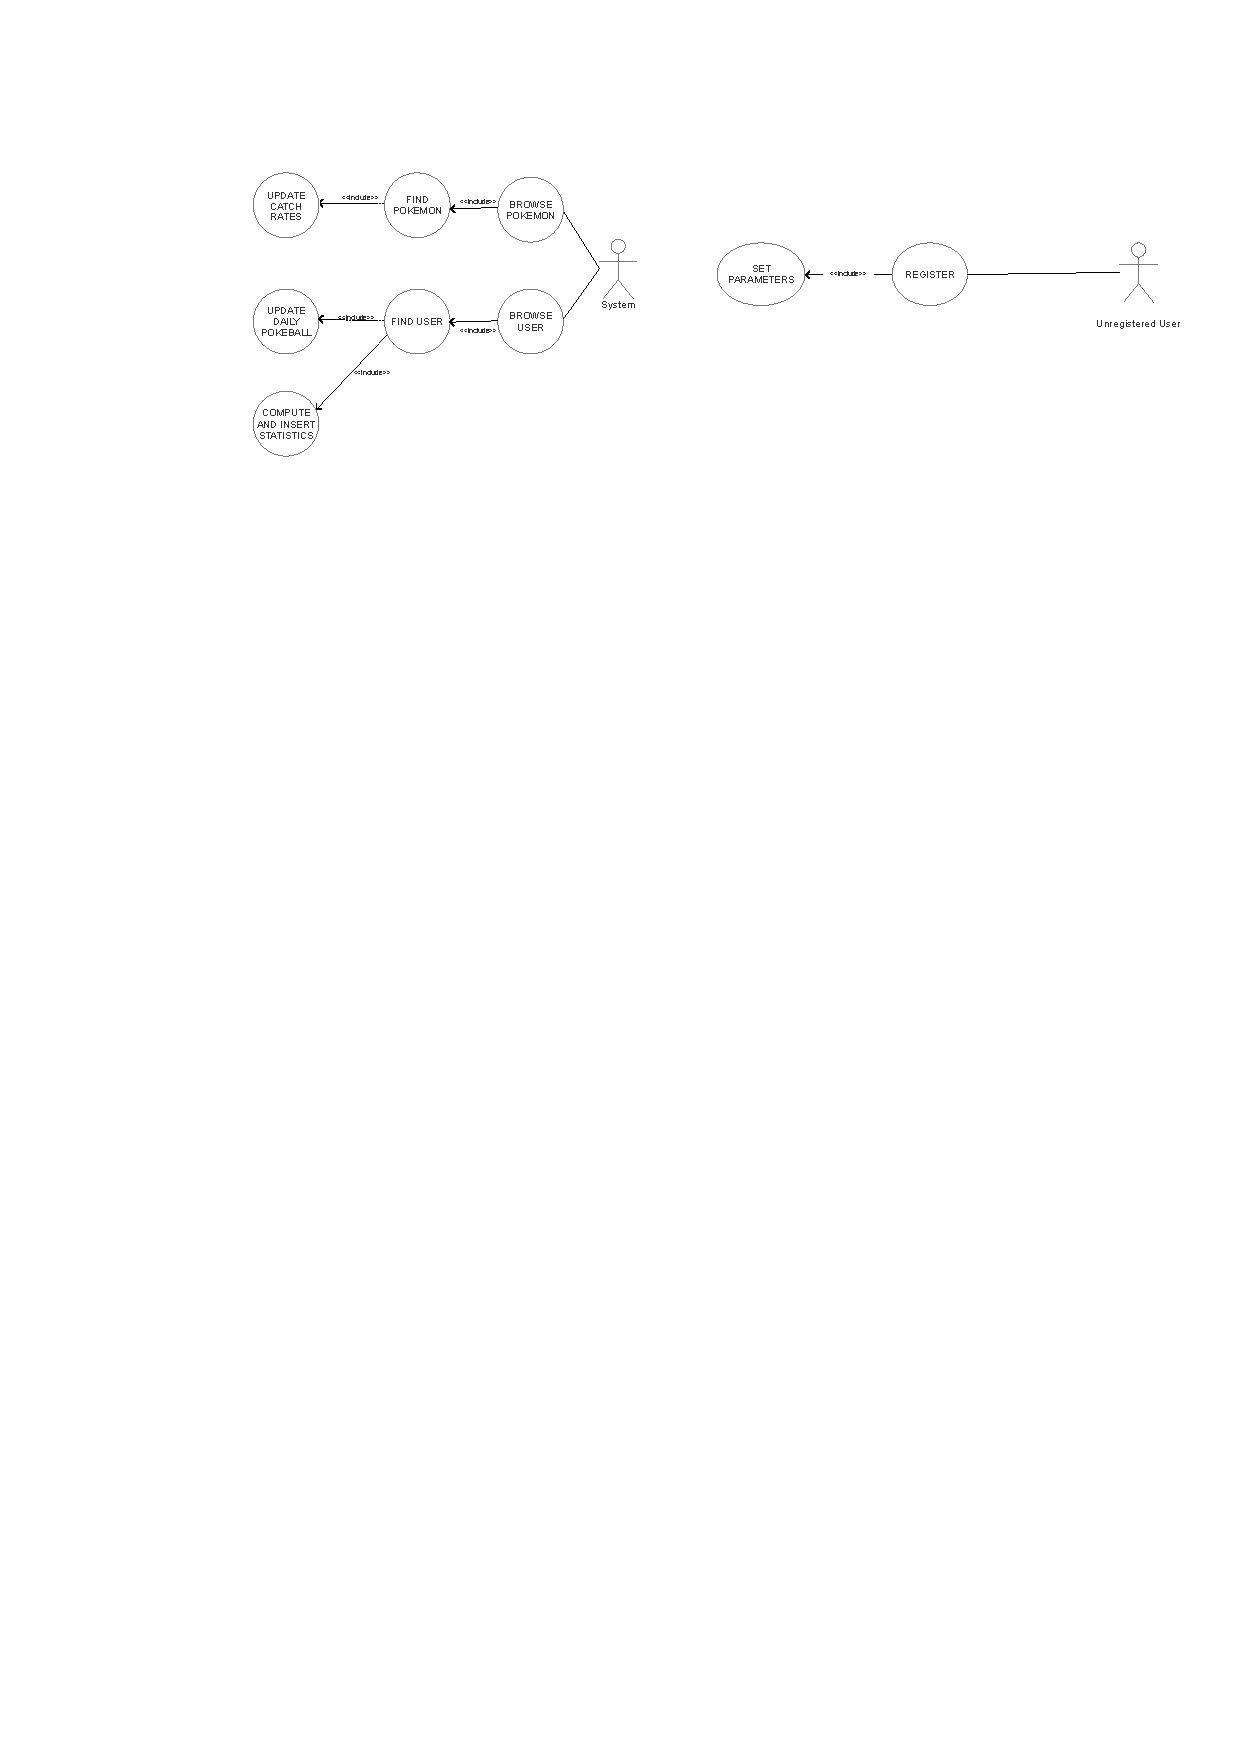
\includegraphics[width=\textwidth]{img/uml_use_case_2.pdf}
	\caption{Use Case Diagram 2}
\end{figure}



\end{figure}
\subsection{Non-Functional Requirements}
\begin{itemize}
	\item The application should guarantee a \textbf{high availability}
	\item It should be \textbf{easy to use}, especially for children and youngsters, and enjoyable
	\item It should have a \textbf{read-your-own-writes consistency} on each \textbf{User}’s own \textbf{Team}, so he/she can always be sure that \textbf{Pokémon} have been correctly caught/freed up
	\item The application should always provide to each \textbf{User} the most recent version of the rankings in order to permit him/her to immediately verify his/her progresses
	\item The statistics regarding usage and \textit{catch rate} evolution are not needed to be real-time, they can be updated periodically and be eventually consistent
	\item \textbf{Posts} and \textbf{Answers} must follow a \textbf{causal-consistency}
	\item \textbf{Response time} is an important issue: redundancies and larger memory consumptions are preferred over high latencies
	\item \textbf{Passwords are crypted} for security reasons
	\item A \textbf{graphical User Interface} and the usage of multimedia are crucial for an involving game experience 
\end{itemize}
\subsection{Sources, Velocity properties and Volume of data}
Data stored in the application backend has been downloaded and imported from the following sources:
\begin{enumerate}
	\item \textbf{Pokèmon Data} $\rightarrow$ \url{https://pokeapi.co},\\ \url{https://bulbapedia.bulbagarden.net/wiki} 
	\item \textbf{Countries data} $\rightarrow$ \url{https://gist.github.com/kalinchernev/486393efcca01623b18d}
	\item \textbf{Data for the generation of realistic users} $\rightarrow$  \url{https://github.com/smashew/NameDatabases/blob/master/NamesDatabases/surnames/all.txt}
\end{enumerate}

All the imported data has been modified, updated and preprocessed in order to satisfy the application needs. 
\textbf{Users} added have the only purpose of showing the application functionalities, \textbf{for privacy issues they are not real people}; anyway, they have been created using \textit{realistic criteria}. \medskip\\
\textbf{Velocity} is guaranteed by the \textit{dynamic catch rate} mechanism: the popularity of a \textbf{Pokémon} influences both its \textit{catch rate} and the amount of \textit{points} that it will provide. As a consequence, \textbf{Users} are continuously stimulated by catching new \textbf{Pokémon}, in order to try to raise their amount of \textit{points}: in this way old \textbf{Teams’} data becomes quickly out-of-date. \\
\textbf{Volume} of data, considering 250K users, almost 1K Pokémon and about 500K posts is no lower than 100Mb.\\
\subsection{UML Entities Diagram}
\begin{figure}[H]
	\centering
	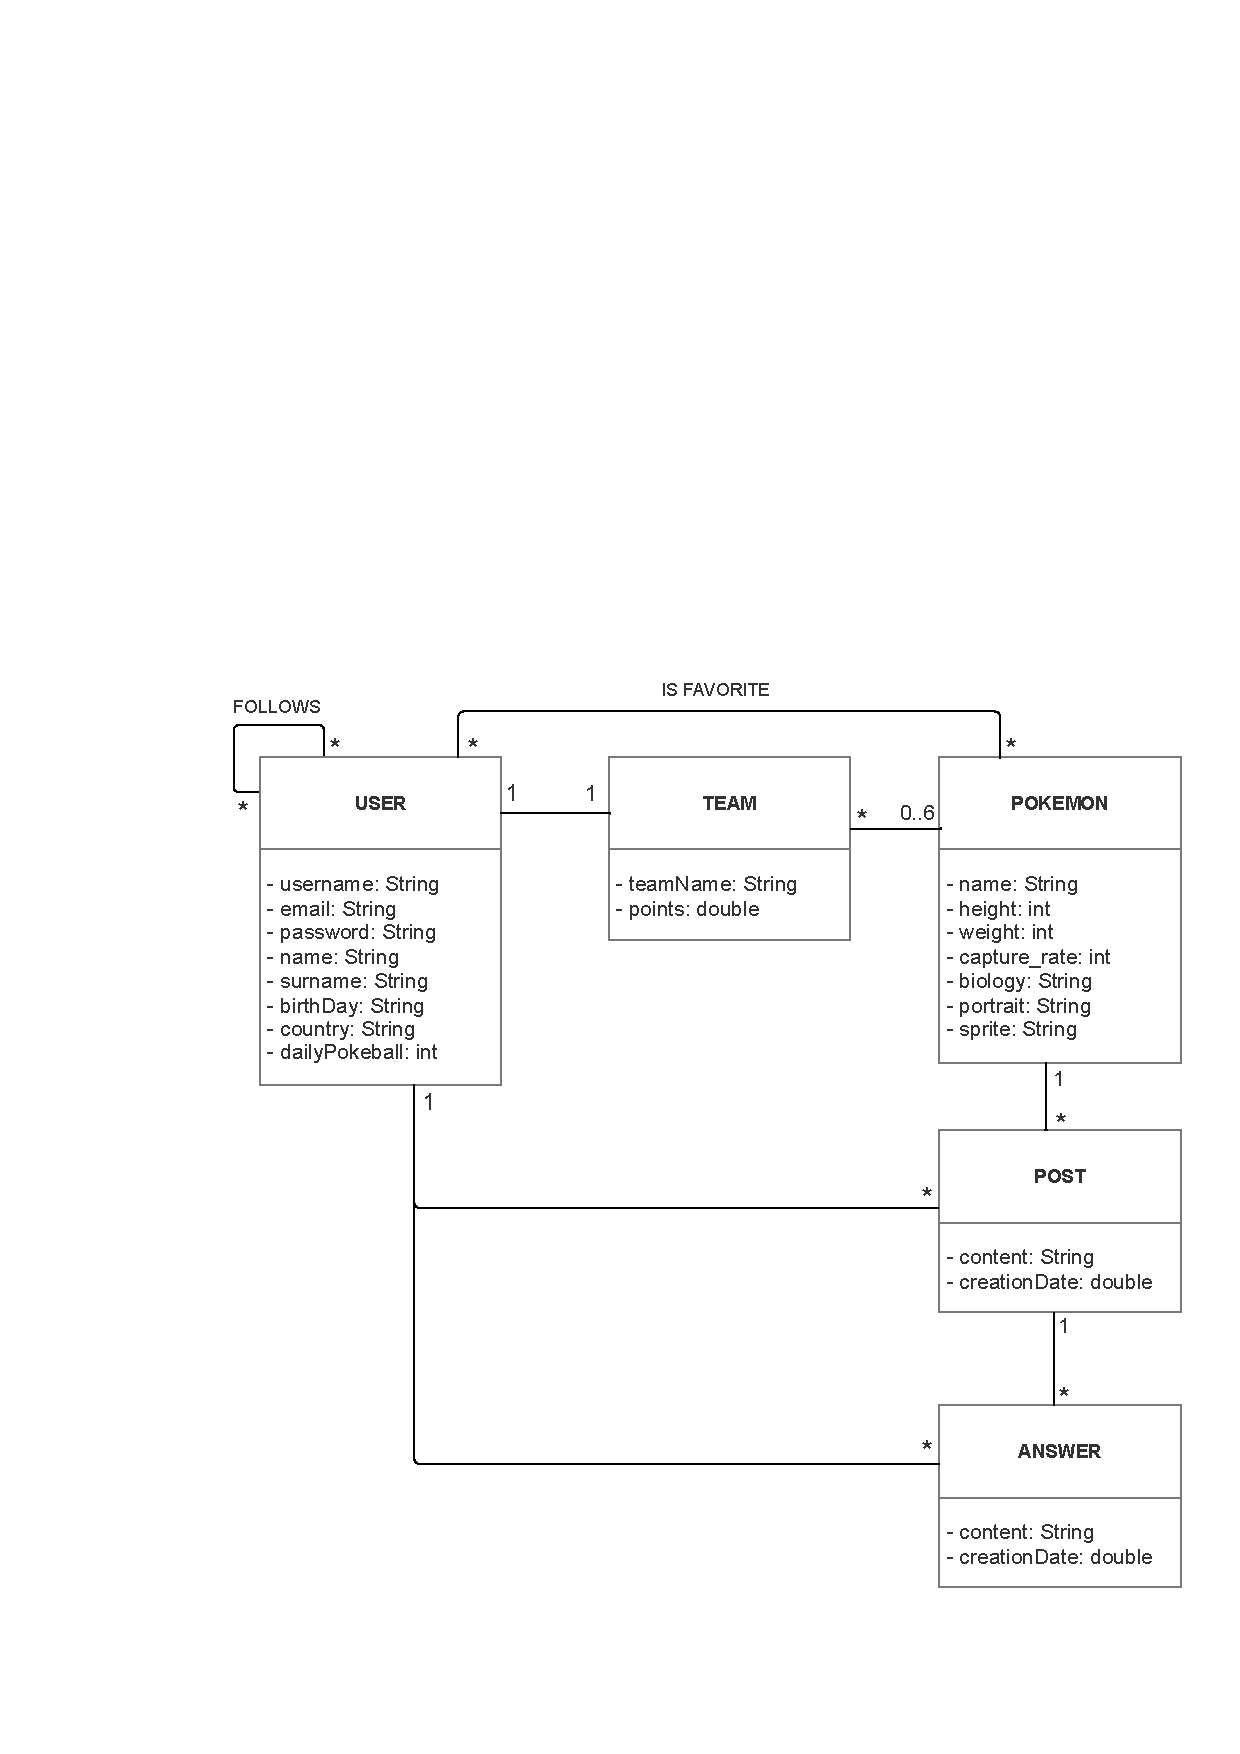
\includegraphics[width=\textwidth]{img/class_diagram.pdf}
	\caption{UML Entity Diagram}
\end{figure}
\begin{enumerate}
	\item A \textbf{User} can build up only one \textbf{Team}: of course, each \textbf{Team} has just one owner.
	\item A \textbf{Team} is composed of a maximum of six \textbf{Pokémons}, every \textbf{Pokémon} can be caught by anyone, so can belong to many \textbf{Teams}.
	\item A \textbf{User} can follow many \textbf{Users}, in the meanwhile he/she can have many followers.
	\item A \textbf{User} can have many favourites \textbf{Pokémon}. A \textbf{Pokémon} can be favourite of many \textbf{Users}.
	\item A \textbf{Post} is created just by one \textbf{User} on one \textbf{Pokémon}. A \textbf{User} can create many posts and a \textbf{Pokémon} can have many \textbf{Posts} talking about it.
	\item An \textbf{Answer} is written by one \textbf{User} and it refers to one \textbf{Post}. \textbf{Users} can submit many Answers and there can be many \textbf{Answers} behind a \textbf{Post}.
\end{enumerate}
\subsection{Main application queries}
\begin{itemize}
	\item Insert a \textbf{User} into the system at registration time
	\item Create a new \textbf{Pokémon} (admin only)
	\item Insert a \textbf{Pokémon} into a \textbf{Team}
	\item Create a new \textbf{Post}
	\item Create a new \textbf{Answer}
	\item Create a follow relationship
	\item Add a \textbf{Pokémon} to the favourites
	\item Retrieve \textbf{User} information at login time
 	\item Retrieve a \textbf{User} by \textit{username }when looking for a new friend
	\item Retrieve \textbf{Team} information based on \textbf{User}
	\item Retrieve \textbf{Pokémon} information using several filters
	\item Retrieve recommended \textbf{Users}
	\item Retrieve list of a \textbf{User}’s friends
	\item Retrieve a \textbf{Pokémon} by \textit{name} when trying to catch it
	\item Retrieve all the \textbf{Posts} relative to a Pokémon
	\item Retrieve all the \textbf{Answers} to a \textbf{Post}
	\item Retrieve \textbf{User}’s favourites \textbf{Pokémons} 
	\item Modify \textbf{User} settings (\textit{email, password, country})
	\item Update \textbf{Team}’s \textit{name}
	\item Update \textbf{Team}’s \textit{points}
	\item Update \textbf{Pokémon}’s \textit{catch rates} Analytics: find $\%$ of \textbf{Users} that own that \textbf{Pokémon}
	\item Remove a \textbf{User} (admin only)
	\item Remove a \textbf{Pokémon} (admin only)
	\item Remove a \textbf{Post} (only admin and post’s owner)
	\item Remove a follow relationship
	\item Remove a \textbf{Pokémon} from the favourite ones
	\item Analytics: ranking of most popular \textbf{Pokémon} in world/each country
	\item Analytics: ranking of best \textbf{Teams} in the world/each country/among friends
	\item Analytics: evolution on time of a \textbf{Pokémon} catch rate
	\item Analytics: evolution on time of number of logins per day/total \textbf{Users}/logins per day by country (admin only)
\end{itemize}

\subsection{Load Estimation}
PokéMongo is an application designed to be spread worldwide and played by plenty of \textbf{Users}. In this paragraph we will try to estimate a realistic computational and memory load, this valuation will be taken into account in the project stage and will be at the foundation of the choices presented in the next chapters

\begin{itemize}
	\item Since the globality of the app and the Social Network structure, we can estimate 5-10M of registered \textbf{Users}. This means about 1M of logins-per-day.
	\item Registered \textbf{Pokémon} are 893. Even though there is the possibility for an admin to add new \textbf{Pokémon}, we think that they will be no more than 1K at every time.
	\item Expert \textbf{Users} will probably generate a higher amount of posts/comments rather than new \textbf{Users}. On average, there will be about 4-5M of \textbf{Posts}/\textbf{Answers} per day.
	\item Beginners are likely to generate an higher load of follow/unfollow requests respect to expert \textbf{Users}. On average, it’s reasonable to count about 5 follow/unfollow requests per login.
	\item Pokéballs and \textbf{Pokémon} capture is the catchiest feature of the game. Very likely almost the totality of the \textbf{Users} that logs into the app will spend all his/her available \textit{daily Pokéballs}. Anyway it’s also probable that the most intriguing \textbf{Pokémon} will be the ones with low \textit{catch rate}. Since there are 10 Pokéballs available each day, but the weighted average probability of catching a \textbf{Pokémon} can be estimated as near 10\%, there will be about 1M of \textbf{Team} updates per day
	\item As said in the previous point, we can count about 10 catch tries per day. It’s likely that the chosen \textbf{Pokémon} was taken from the provided favourite shortcut. Moreover, likes are integrating part of this Social Network, not only a practical tool for catching \textbf{Pokémon}. So we can say that there will be about 2M of likes per day.
	\item We can estimate that on the average a \textbf{User} will consult \textit{Ranking} twice per day. Indeed immediately after log in and at the catching of a new \textbf{Pokémon} are possible occasions in which the user could be interested in seeing his/her progresses. For this reason we can consider 2M of ranking consulting per day
	\item Very few \textbf{Users} will change his/her settings or password, since they are long term fields: this kind of updates will be no more than 30-40K per day.
\end{itemize}

